% !TEX TS-program = pdflatex
% !TEX encoding = UTF-8 Unicode

% This is a simple template for a LaTeX document using the "article" class.
% See "book", "report", "letter" for other types of document.

\documentclass[11pt]{article} % use larger type; default would be 10pt

\usepackage[utf8]{inputenc} % set input encoding (not needed with XeLaTeX)

%%% Examples of Article customizations
% These packages are optional, depending whether you want the features they provide.
% See the LaTeX Companion or other references for full information.

%%% PAGE DIMENSIONS
\usepackage{geometry} % to change the page dimensions
\geometry{a4paper} % or letterpaper (US) or a5paper or....
% \geometry{margin=2in} % for example, change the margins to 2 inches all round
% \geometry{landscape} % set up the page for landscape
%   read geometry.pdf for detailed page layout information

\usepackage{graphicx} % support the \includegraphics command and options
\usepackage{grffile}

% \usepackage[parfill]{parskip} % Activate to begin paragraphs with an empty line rather than an indent

%%% PACKAGES
\usepackage{booktabs} % for much better looking tables
\usepackage{array} % for better arrays (eg matrices) in maths
\usepackage{paralist} % very flexible & customisable lists (eg. enumerate/itemize, etc.)
\usepackage{verbatim} % adds environment for commenting out blocks of text & for better verbatim
\usepackage{subfig} % make it possible to include more than one captioned figure/table in a single float
% These packages are all incorporated in the memoir class to one degree or another...

%%% HEADERS & FOOTERS
\usepackage{fancyhdr} % This should be set AFTER setting up the page geometry
\pagestyle{fancy} % options: empty , plain , fancy
\renewcommand{\headrulewidth}{0pt} % customise the layout...
\lhead{}\chead{}\rhead{}
\lfoot{}\cfoot{\thepage}\rfoot{}

%%% SECTION TITLE APPEARANCE
\usepackage{sectsty}
\allsectionsfont{\sffamily\mdseries\upshape} % (See the fntguide.pdf for font help)
% (This matches ConTeXt defaults)

%%% ToC (table of contents) APPEARANCE
\usepackage[nottoc,notlof,notlot]{tocbibind} % Put the bibliography in the ToC
\usepackage[titles,subfigure]{tocloft} % Alter the style of the Table of Contents
\renewcommand{\cftsecfont}{\rmfamily\mdseries\upshape}
\renewcommand{\cftsecpagefont}{\rmfamily\mdseries\upshape} % No bold!

%%% END Article customizations

%%% The "real" document content comes below...

\title{Effect Estimation Project}
\author{Brandon Avila}
%\date{} % Activate to display a given date or no date (if empty),
         % otherwise the current date is printed 

\begin{document}
\maketitle

\section{}
The methods outlined here aim to detect the effect of an unknown rare protective variant using only control data. Simulations were based on a model of genetic variance with a specified heritability of disease, and fractions of this heritability explained by known common variants, unknown common variants, and unknown rare variants.

\section{}
IAll methods were performed on sets of 500000 simulated individuals, a disease with $h^2 = 0.3$, baseline prevalence 0.1, and 200 common known-effect variants with 2 rare unknown-effect variants. Rare variants were always protective with frequency 0.005 and effect size -1.23 unless otherwise specified here. Each study only estimates the effect of one of the variants, namely, $\beta_{201}$.

\subsection{Method A}
This method takes cases and controls and assumes we have information on all of the individuals. It simply compares the prevalence of disease in those with one protective allele to that in those with zero protective alleles. With only the individuals I generated (significantly fewer cases than controls), I took this to be a decent estimate of our best guess on the effect size. The assumption here was that if the method gave an inaccurate estimate, it probably was because we didn't get enough cases or enough individuals with the protective allele or something like that. While less optimal than performing a true case-control study, this gave reasonable results, and was held as the "silver standard" for the rest of my tests (that is, the best way to fake a real analysis).

\subsection{Method B}
Here, we select out the healthy individuals (as we assume we only have controls). Then we do a linear fit of $\widehat{PRS}$ to genotype. Here, the slope should be the negative of $\hat{\beta}_{201}$.

\subsection{Method C}
This method was an attempt to do something similar to Method B with cases rather than controls, but I abandoned this idea and just stuck with all control-based tests. No results from this method.

\subsection{Method D}
Essentially, this is a pseudo-case-control study on the tails of the $\widehat{PRS}$ distribution of the healthy individuals. Take the top and bottom tails (tail size can be altered, but commonly 10\%), and compare the "prevalence" of disease in those with zero, one, and two allele genotypes for our rare variant. If no individuals in the tails have genotype 2, we discard the result, as two points cannot give us a p-value, so the estimate is not meaningful. Then, translate the prevalences into risk scores, and do a linear fit on the scores vs genotypes. If the prevalence in those with genotype $G_{201} = 2$ is 0 or 1, the score for that point is $\pm \infty$, so the linear fit will make no sense, and the estimate is not meaningful.

For this method, only the estimates that did not fail in either of those ways were included in the results.

\subsection{Method E}
Perform Method B, but rather than fitting the entire $\widehat{PRS}$ distribution to the genotypes, select out only the middle 50\% of the distribution for each genotype. The thought here was that we would still maintain a distribution of $\widehat{PRS}$ for each genotype, but would not allow outliers to contribute as much to the estimate.

\subsection{Method F}
Perform Method D, but instead of using three equally weighted points, weight each genotype point by the number of individuals (in the tails) with that genotype. Now, for example, a prevalence estimate from one person with $G_{201}=2$ should count for less than a prevalence estimate from 15000 people with $G_{201}=0$.

\section{}
I did a lot of playing with things and tweaking parameters, so this is just a rundown on how the methods compare, and what I think the best choices are.

\subsection{B-E Comparison}
Obviously we need to do a comparison of these two, since E is a variation on B.

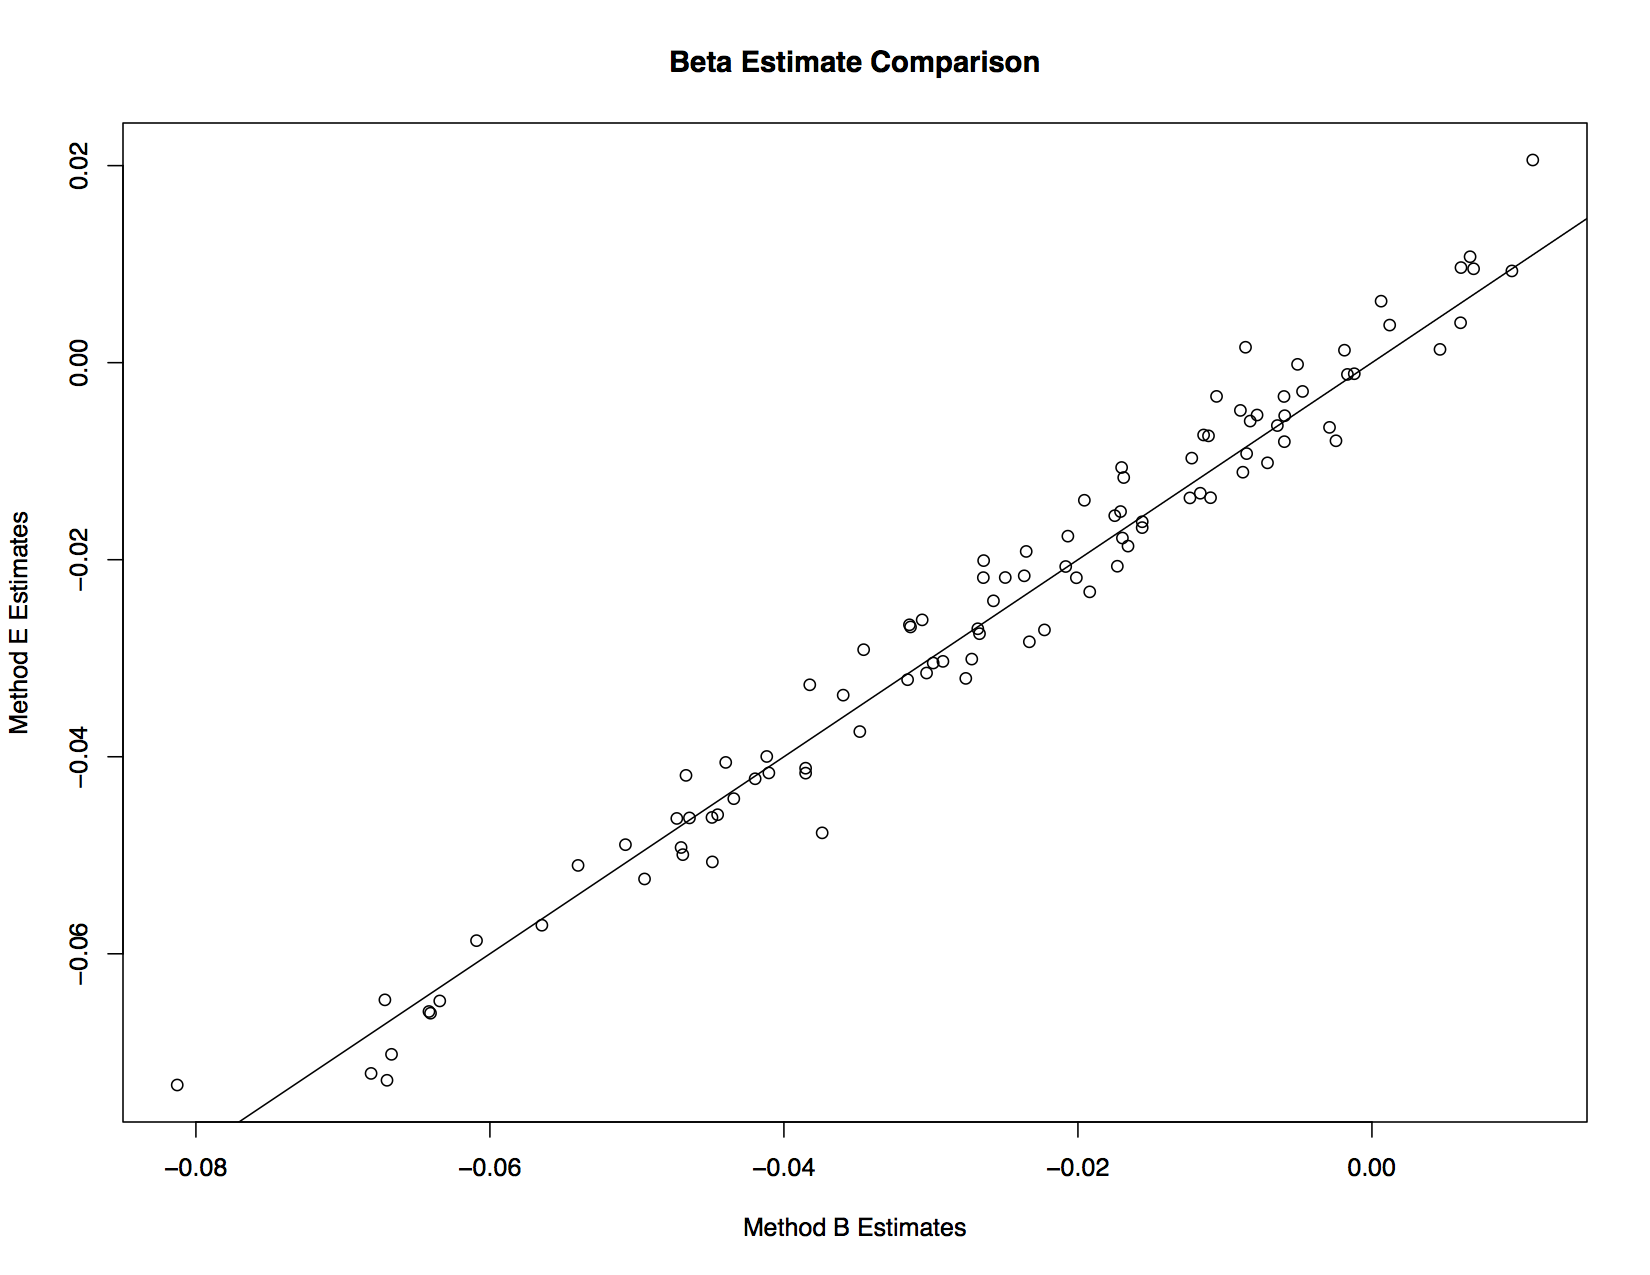
\includegraphics[scale=0.5]{BE Comparison.png}

The above figure has estimates from B and E on 100 tests. My takeaway from this figure was that it basically doesn't matter whether we use B or E. For me, it was actually more computationally intensive to select out the middle 50\% of the distributions rather than just run them all through the fit, so I rejected E and used B from here on out.

\subsection{Method B p-Values}

It was important to check the p-Values on the estimates from Method B to see when we could definitively say that we had detected an effect, and make sure that when we did, we had at least the right sign. It turns out that the relation between p-Value and estimate was super super strong.

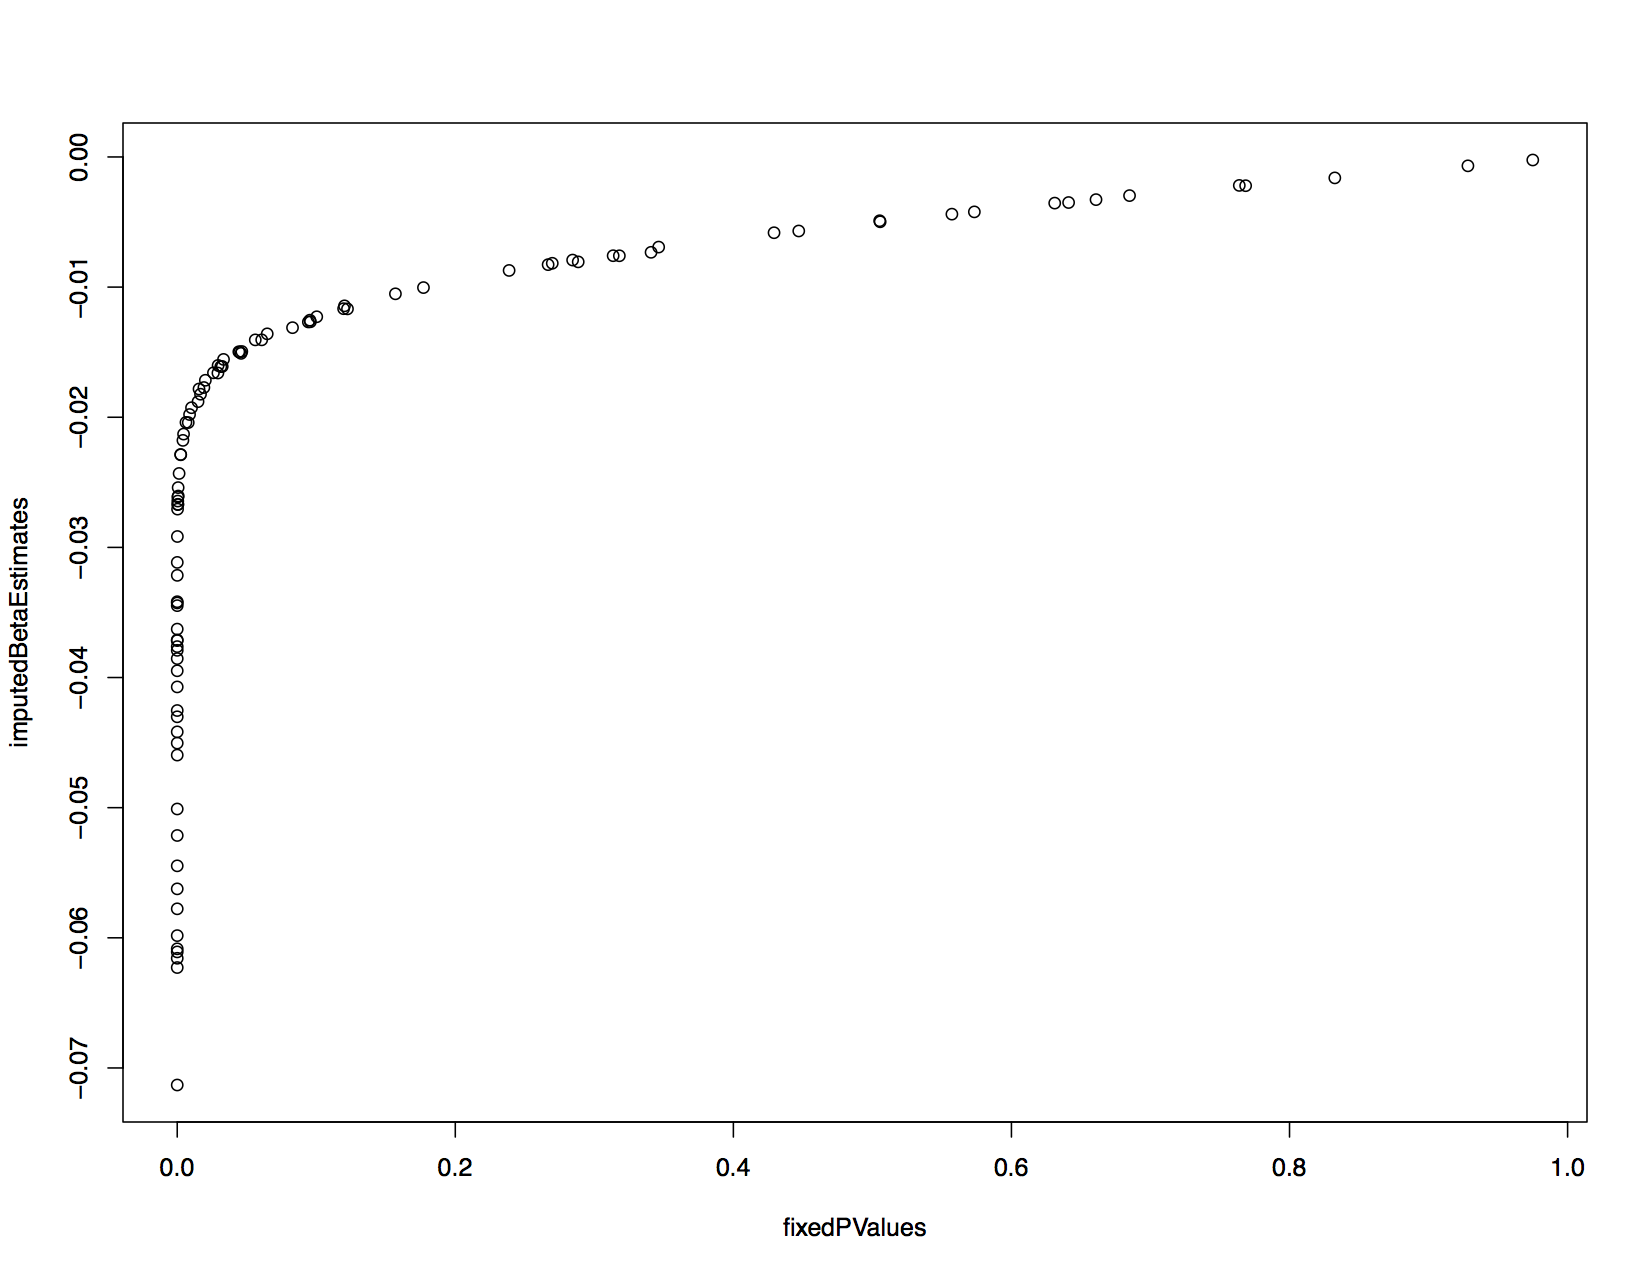
\includegraphics[scale=0.5]{Beta Estimates vs p-Value.png}

Sorry for the bad axis labels. This particular graph actually included some estimates that were positive (there were one or two between p-values 0.6 and 1.0), but I flipped them over the x-axis, and they fit right along with this curve. I also excluded one or two outliers. I have no idea what's going on here. I became briefly obsessed with trying to fit this curve, thinking that if I found the y-intercept, I would have a really good estimate of $\beta_{201}$. It turns out that it's not a very easy curve to fit, so I sort of gave up on that eventually.

Anyway, all the points with $p<0.5$ had the right sign, so this method is at least pretty good at detecting that.

\subsection{D-F Comparison}
This is the next natural comparison to make, since F is a variation on D.

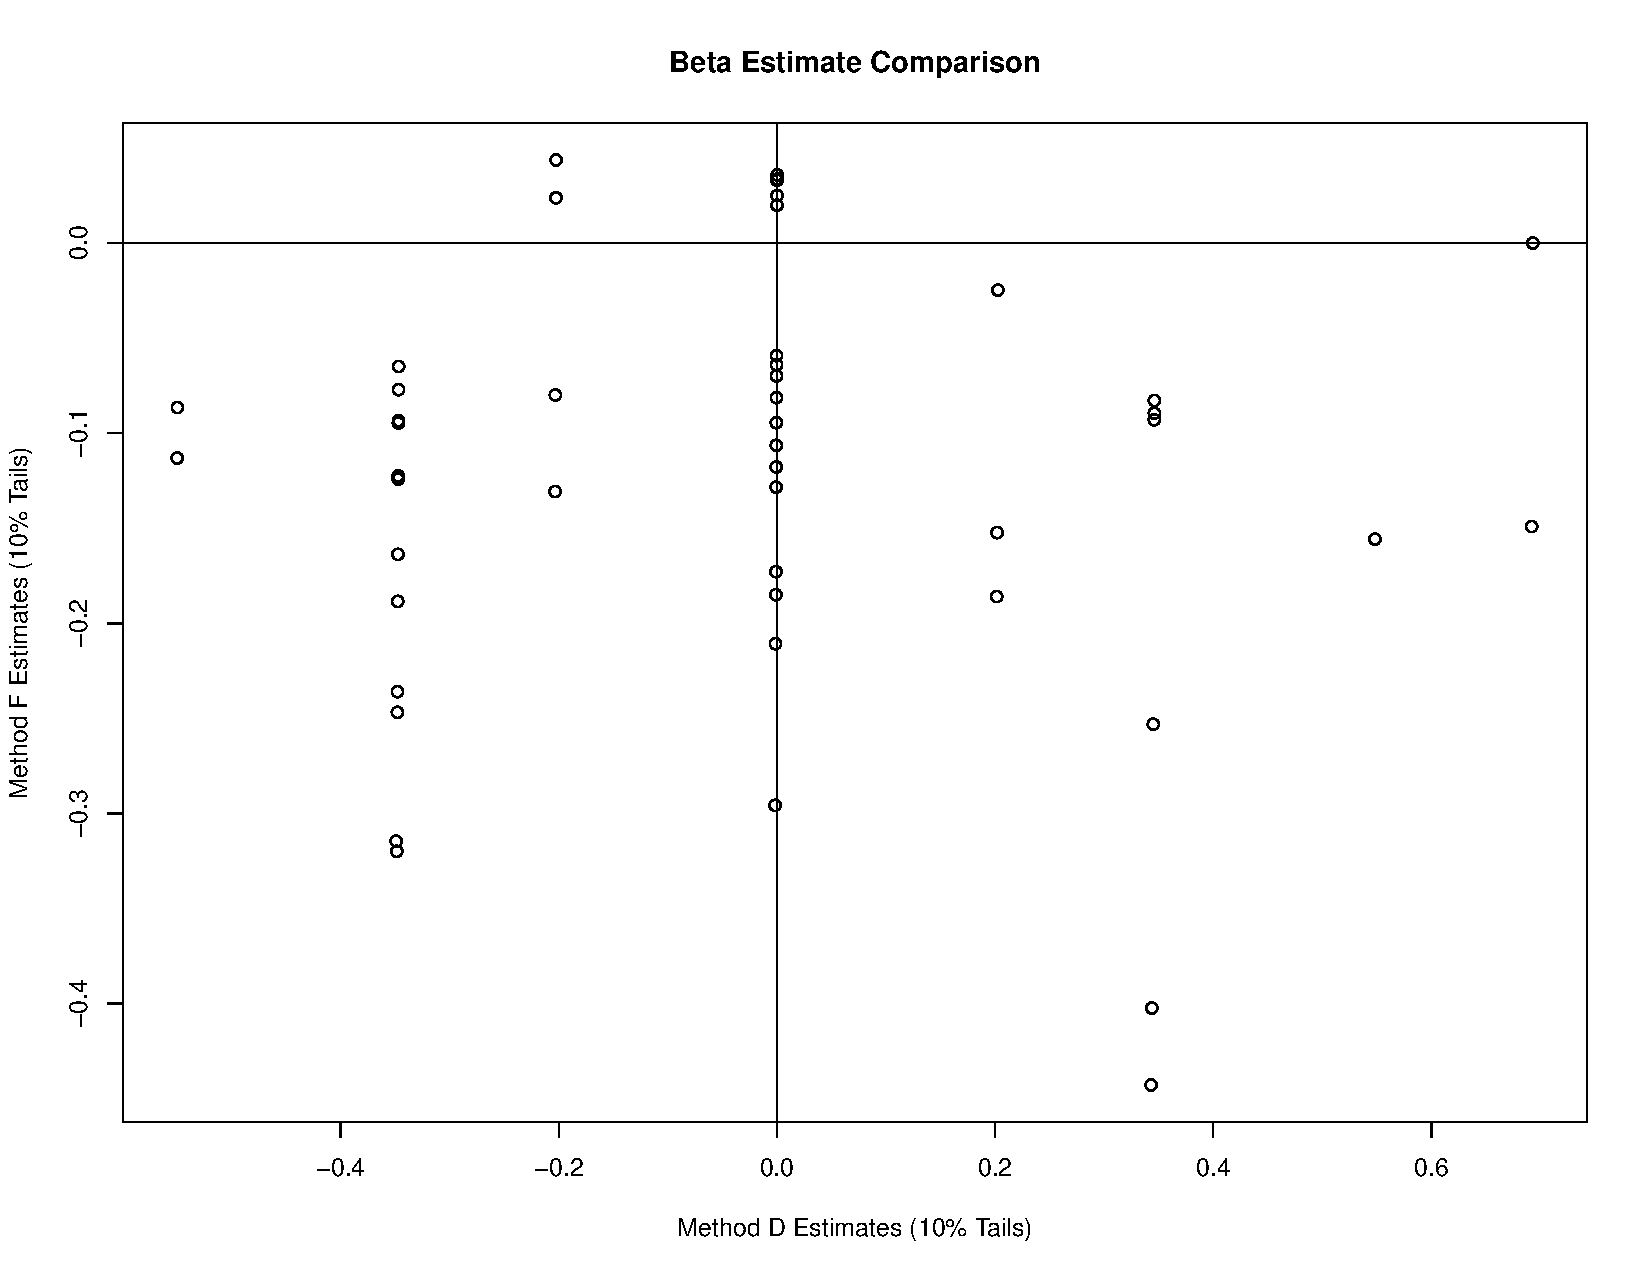
\includegraphics[scale=0.5]{DF Comparison (10Percent).pdf}

The comparison here shows that in general, Method F gives more accurate sign detection than Method D. The p-values are similar, being uniformly slightly lower for Method F, but I don't have a graph of that. I decided, based on this graph and the similar p-values, that Method F was better than Method D for detecting the sign of the effect, and rejected D in favor of F.

\subsection{Tail Size}
Deciding on the tail size is a trade-off between statistical power and the ability to actually come up with a result that isn't rejected based on the criteria listed under the description of Method D.

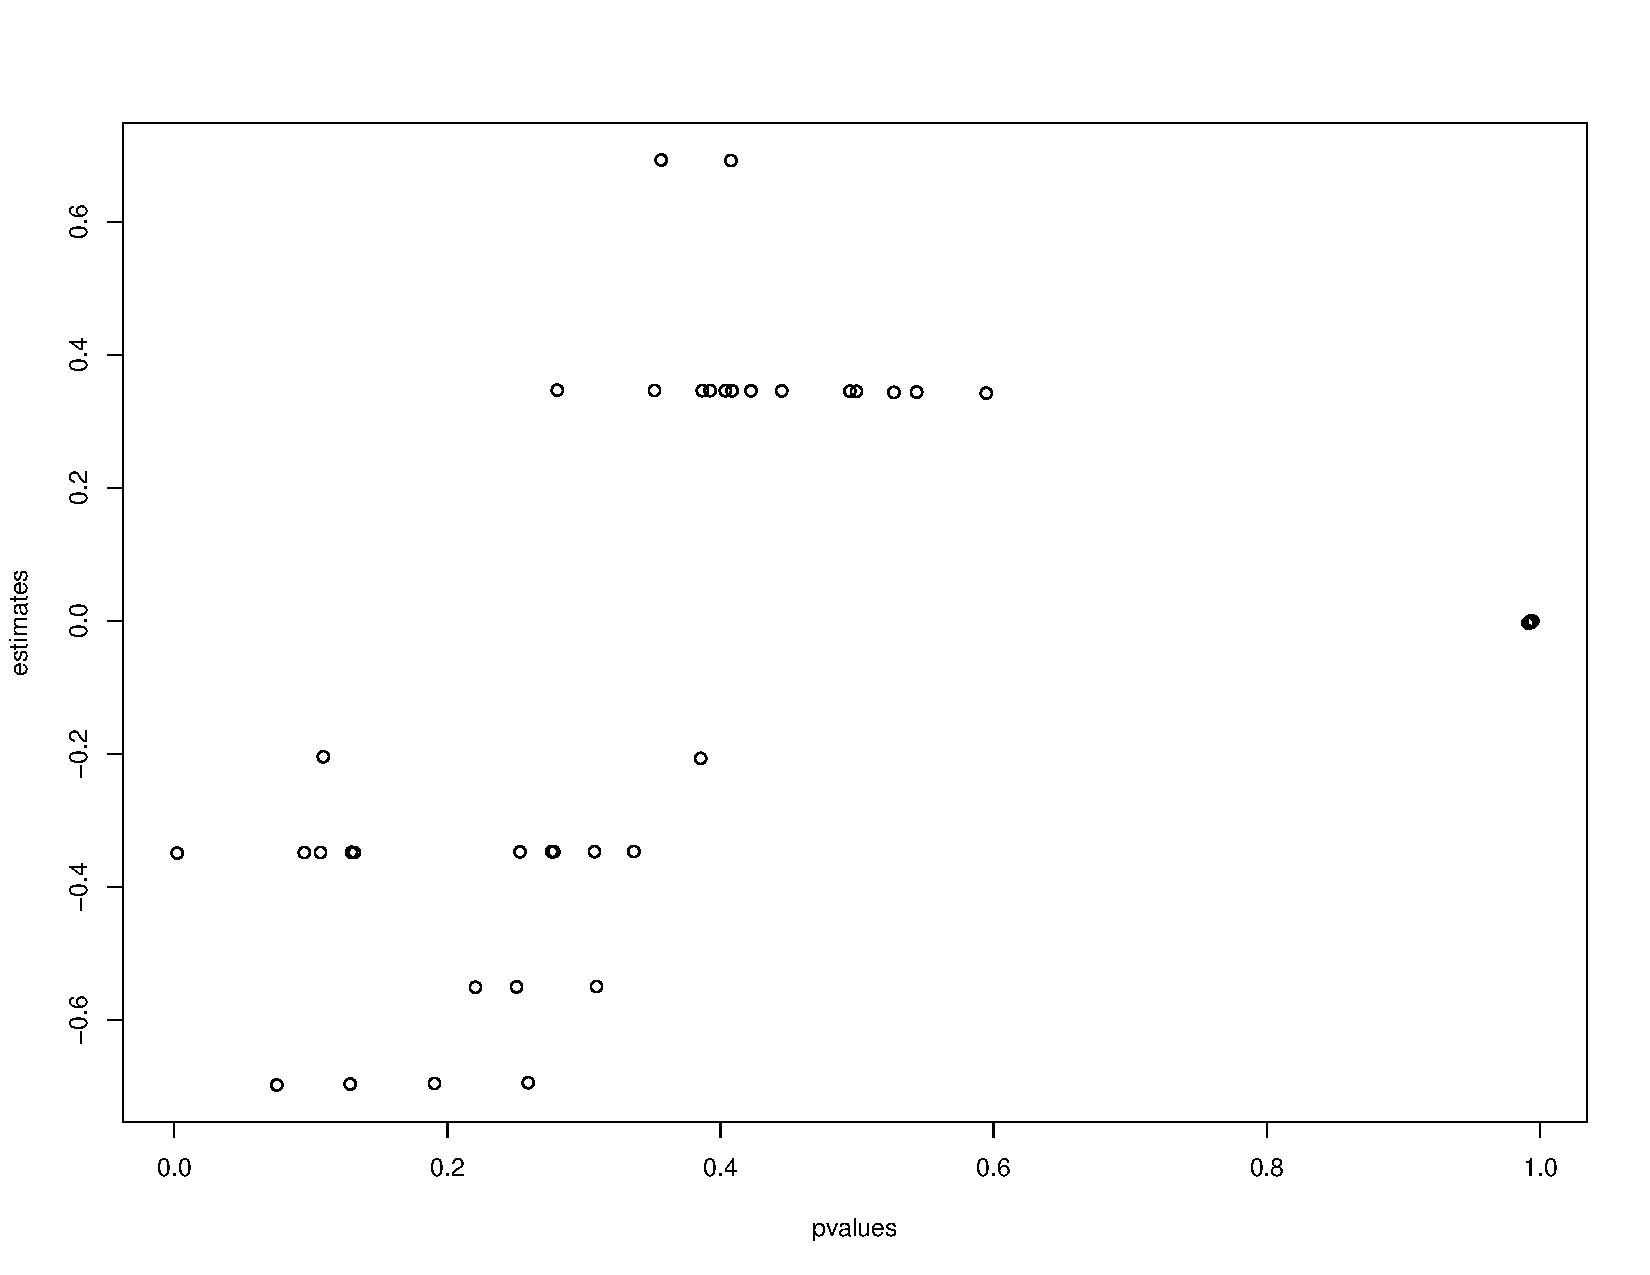
\includegraphics[scale=0.25]{Method D 10Percent Tails.pdf}
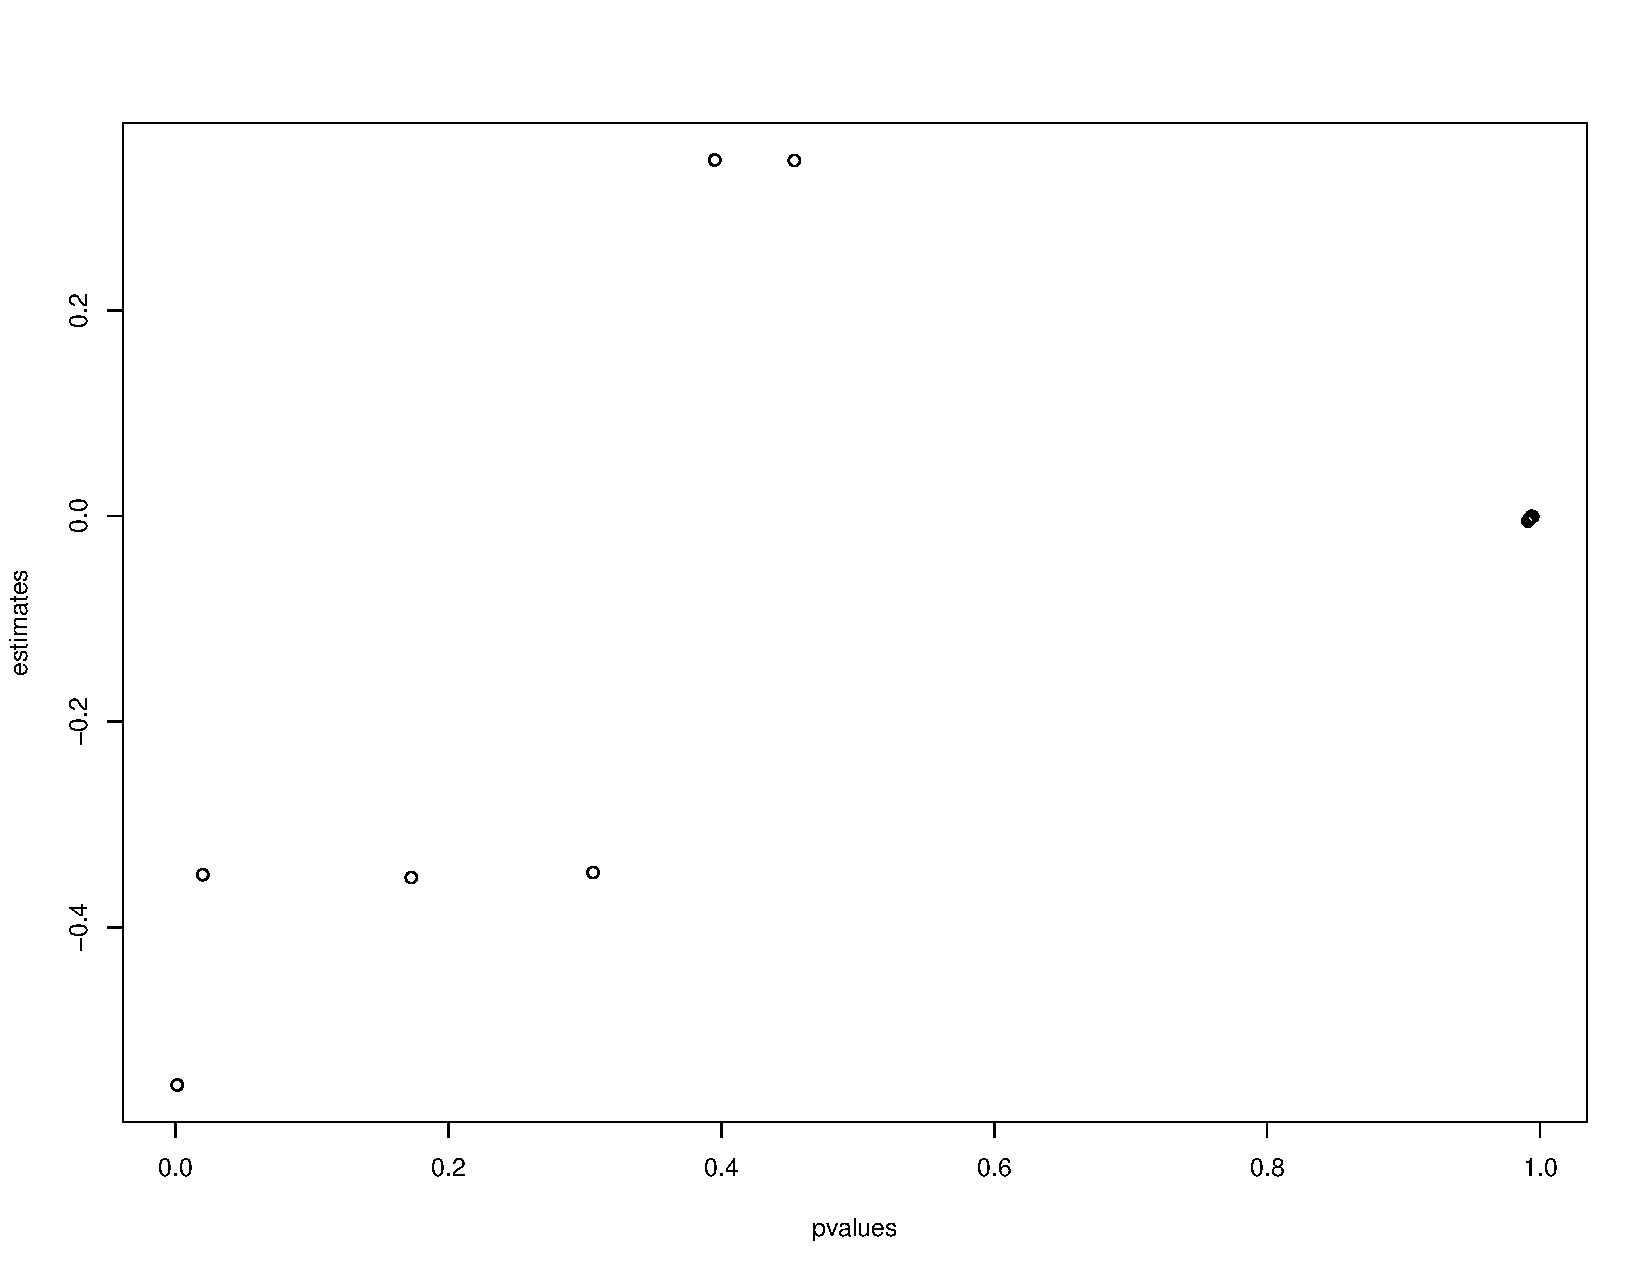
\includegraphics[scale=0.25]{Method D 5Percent Tails.pdf}

In both of the above graphs, 100 tests were done, and only those results that met the aforementioned criteria were kept. The one on the left used 10\% tails, and the one on the right used 5\% tails. Because the spread of p-values were pretty similar, and for sufficiently low p-values, the estimates were the same, I decided that using 10\% tails was better than using 5\%, since we could get meaningful estimates way more often. I didn't look into using even bigger tails, but I wonder how big we would have to make the tails before this became ineffective.

\subsection{B-F Comparison}
I decided that B was easier to use than E, and F gave better results than D, so the last thing to do was to compare B and F.

First, I tried 100 tests to compare B to F and to look at their power for detecting effects.

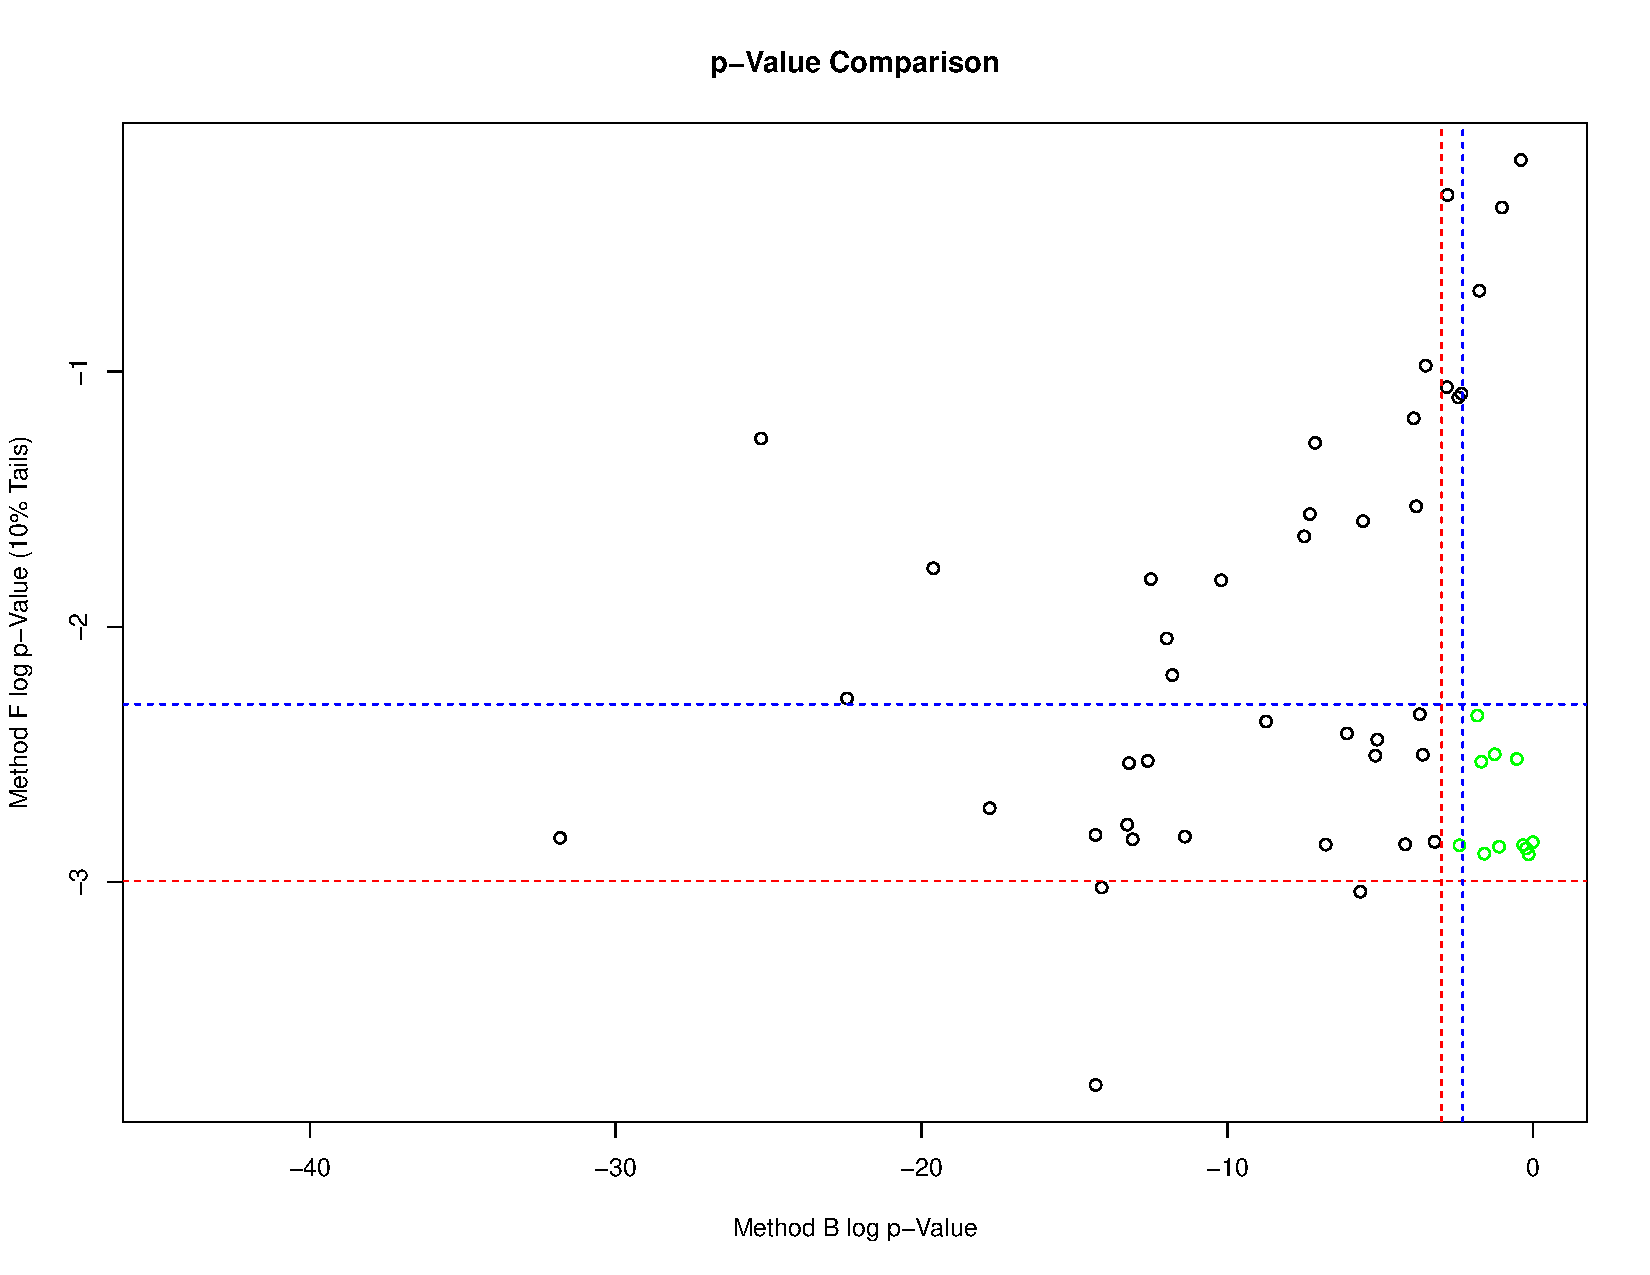
\includegraphics[scale=0.5]{BF Comparison Comprehensive p.pdf}

In the above graph, the p-values for Methods B and F are compared for the tests for which Method F produced a meaningful result. The blue lines represent a p-value of $p=0.10$, and the red lines represent $p=0.05$. The green highlighted points are those for which (given \emph{some} p-value) Method F may detect while Method B does not (that is, $p_F < p_B$.

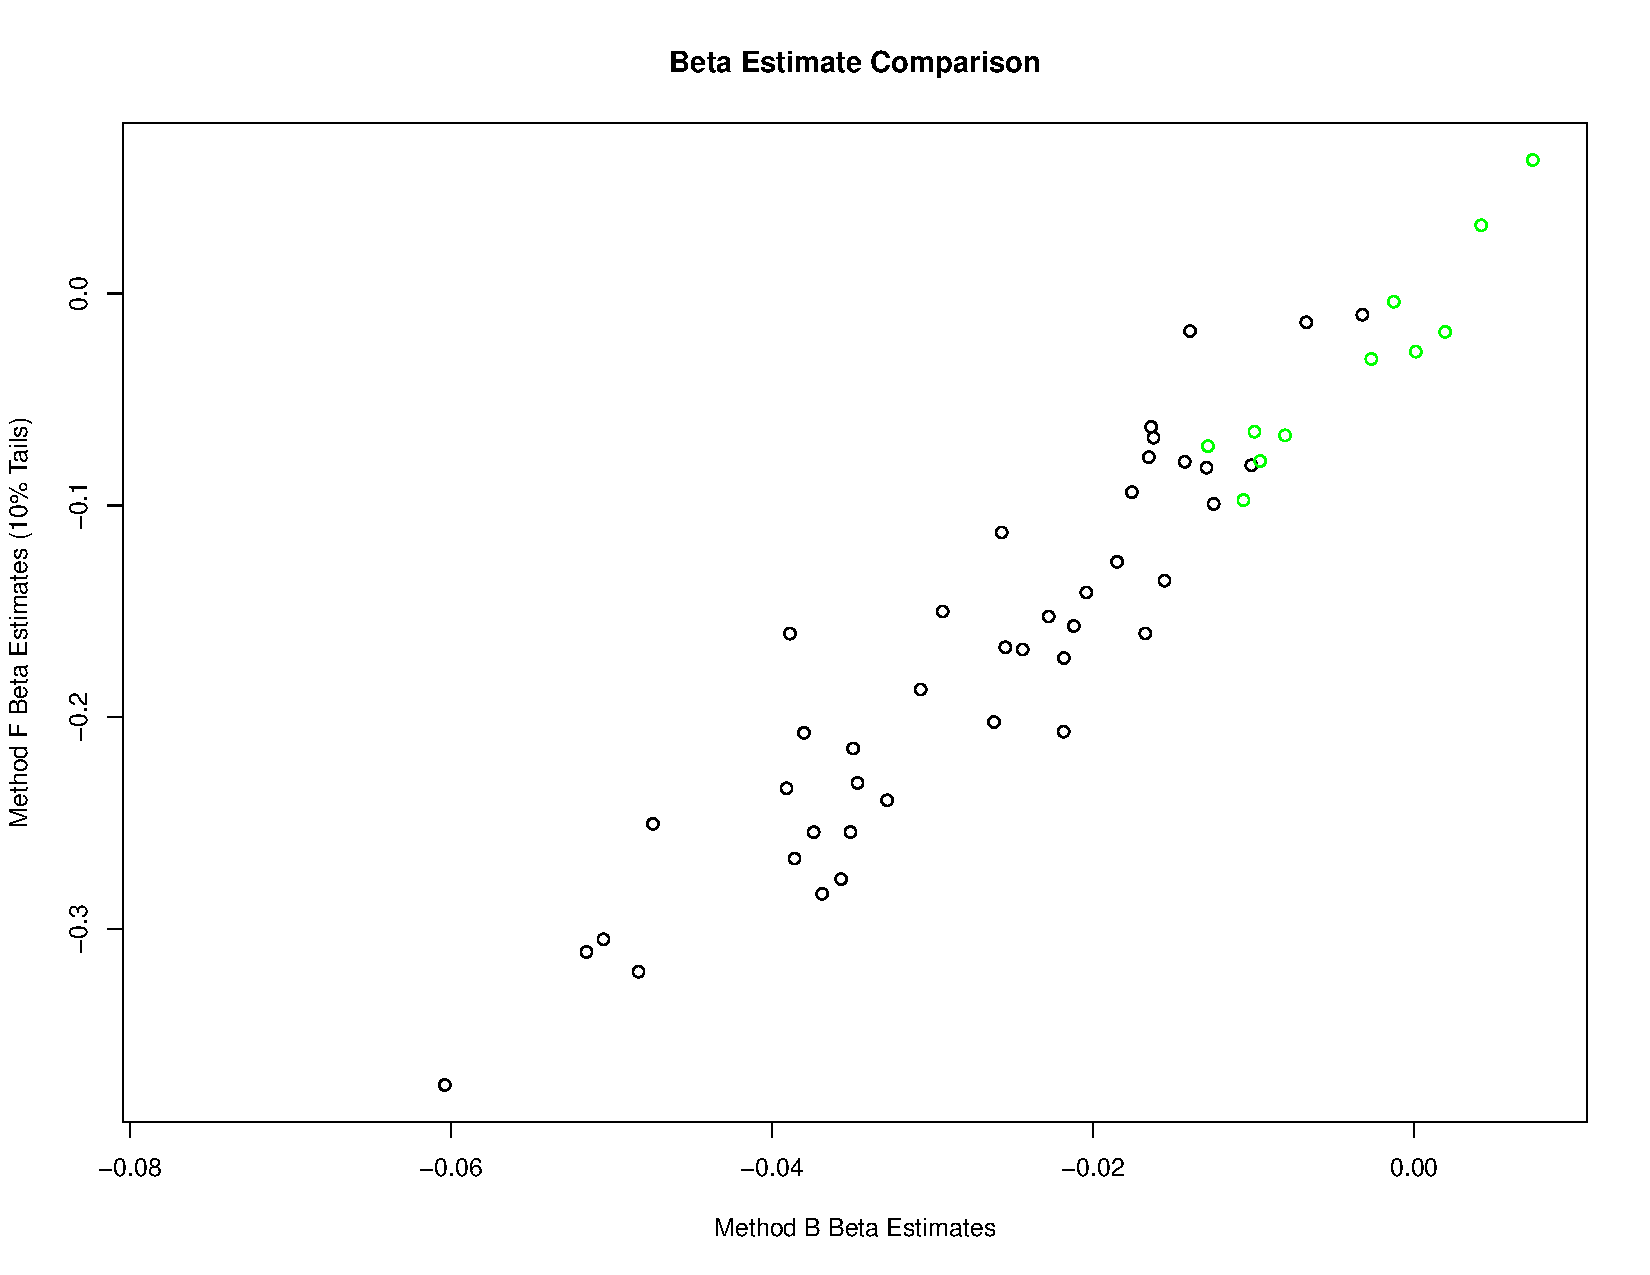
\includegraphics[scale=0.5]{BF Comparison Comprehensive.pdf}

I plotted the actual estimates to see where these green points fell. While not detected at $p=0.05$, many of these green points were detected by Method F at $p=0.10$. It seems that when using Method F, in order to have a significant rate of effect detection, we need to adjust the p-value such that we end up with many false sign errors. Nevertheless, it's interesting to note that estimates from B and F do correlate linearly, and an extreme estimate from Method F corresponds to an extreme estimate from Method B, which in turn has a low p-value. It is possible that Method F is more useful than its reported p-values lead us to believe.

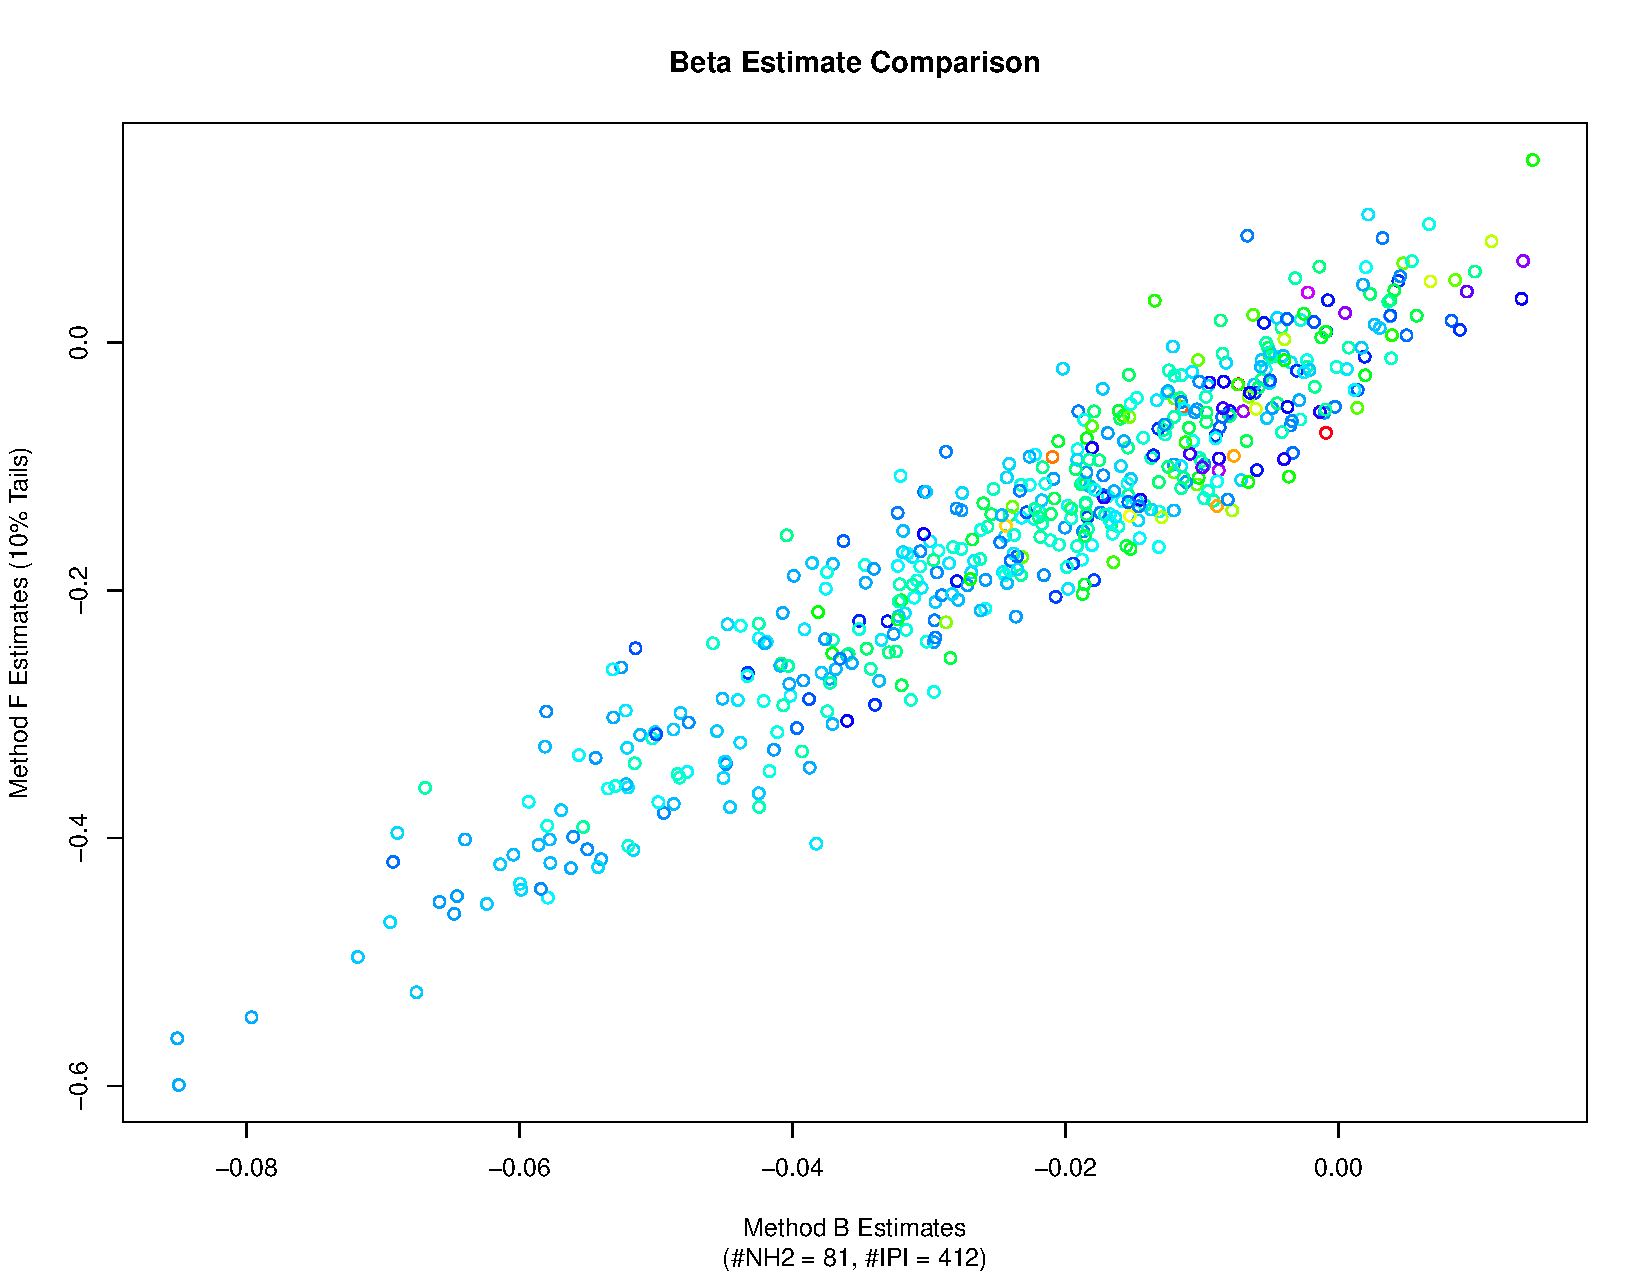
\includegraphics[scale=0.5]{ABF Comparison Big.pdf}

Above is a plot of the estimates from Methods B and F over 1000 simulations. The colors correspond to the estimates provided by Method A with reds and purples being the most extreme estimates. It's a bit puzzling at first why more extreme estimates from A on \emph{both} sides correspond to closer-to-zero estimates for Methods B and F, but this is likely because these extreme estimates come from less favorably distributed data.

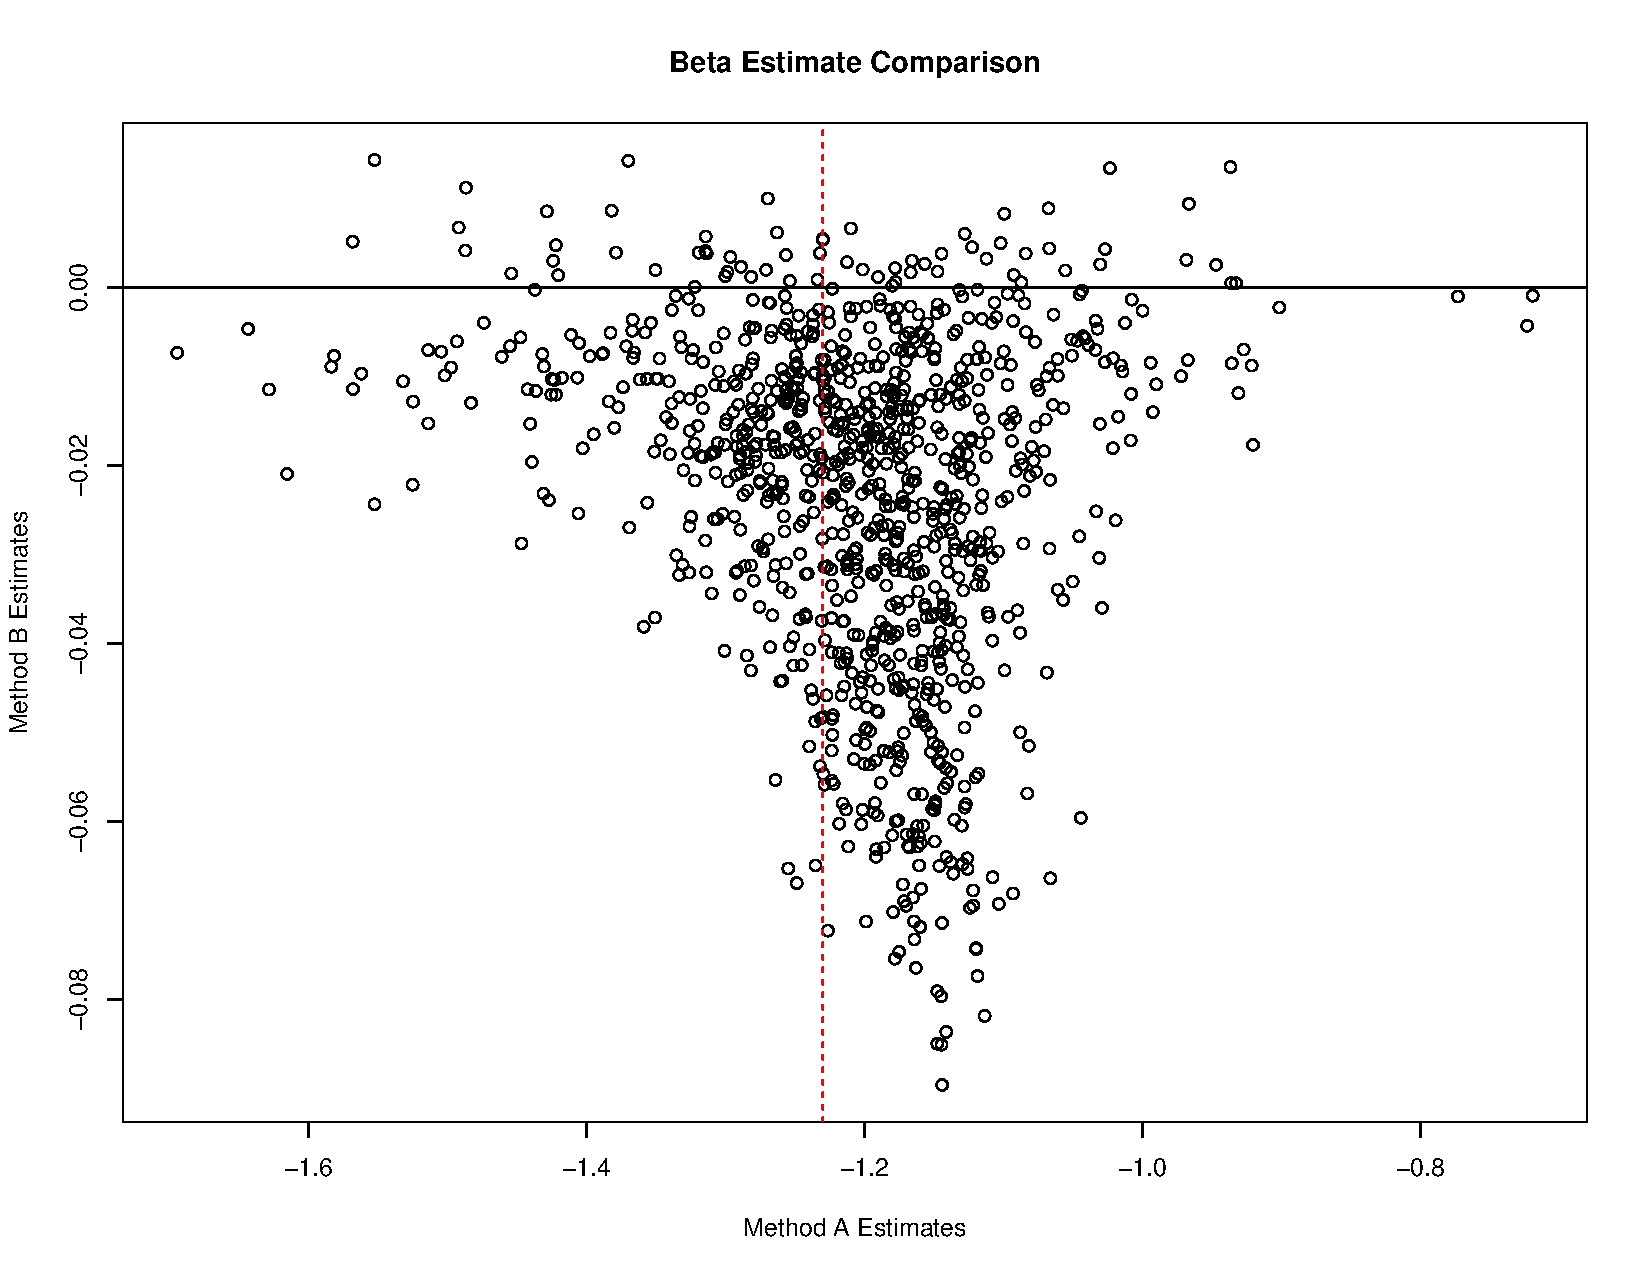
\includegraphics[scale=0.5]{AB Comparison Big.pdf}

Here, I plotted just the B estimates against the A estimates. The shape is a bit confusing, since the red line is the true value of $\beta_{201}$. I'm not sure why we get the lowest estimates (and hence, best p-values) when A decides to estimate a little above the true effect size.

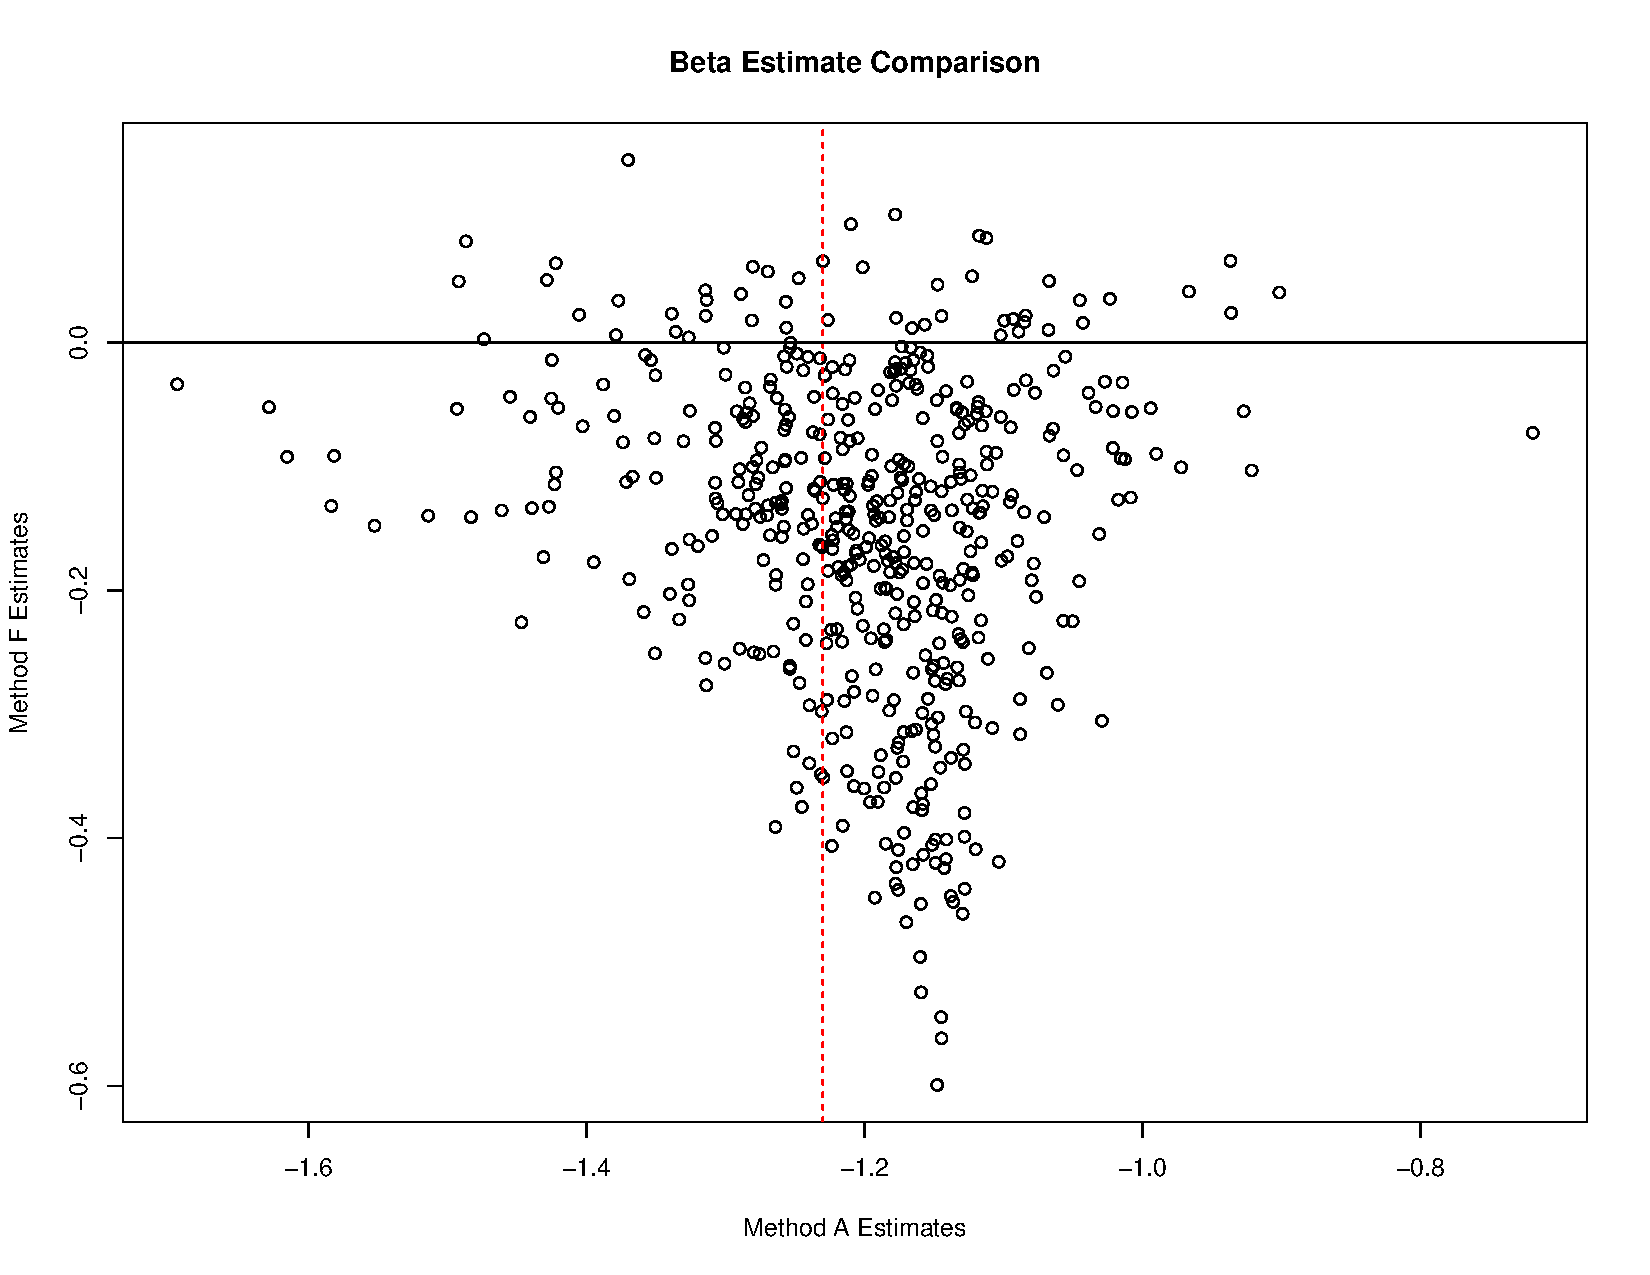
\includegraphics[scale=0.5]{AF Comparison Big.pdf}

This is F vs A. Fewer points because a lot of them got rejected, but still the same shape, which is to be expected, as B and F are pretty linear.

\section{}

Ultimately, I chose not to consider the method where we simulate cases and controls by coin-flipping from $\widehat{PRS}$ because every individual has such a similar estimated score that I expect it wouldn't give a detectable effect unless we had an obscene number of individuals.

FInally, it looks like Method B is the easiest and most consistent way to predict sign. Method F gives a better order of magnitude estimate, but because it's pretty linear with respect to B, it doesn't really give any additional information. If we could figure out what was going on with the p-values in B, maybe we could find a way to get a more accurate magnitude of estimate, but as I mentioned, I tried and it's hard.

I want to try estimating multiple effects at once. My plan for this is to use Method B, but instead of regressing on just one genotype variable, regress on many. This should reduce effects from covariance in genotypes.

\section{}

Taking the analysis a step further, I tested Method B's response to changing the heritability explained by altering the frequency and effect sizes of the rare variants. Here, recorded effect size estimates and p-values as changes were made in both of these directions.

\includegraphics[scale=0.5]{Understanding B/Constant MAF.pdf}

Here, I hold the allele frequency of the rare variants constant, and alter their effect sizes.

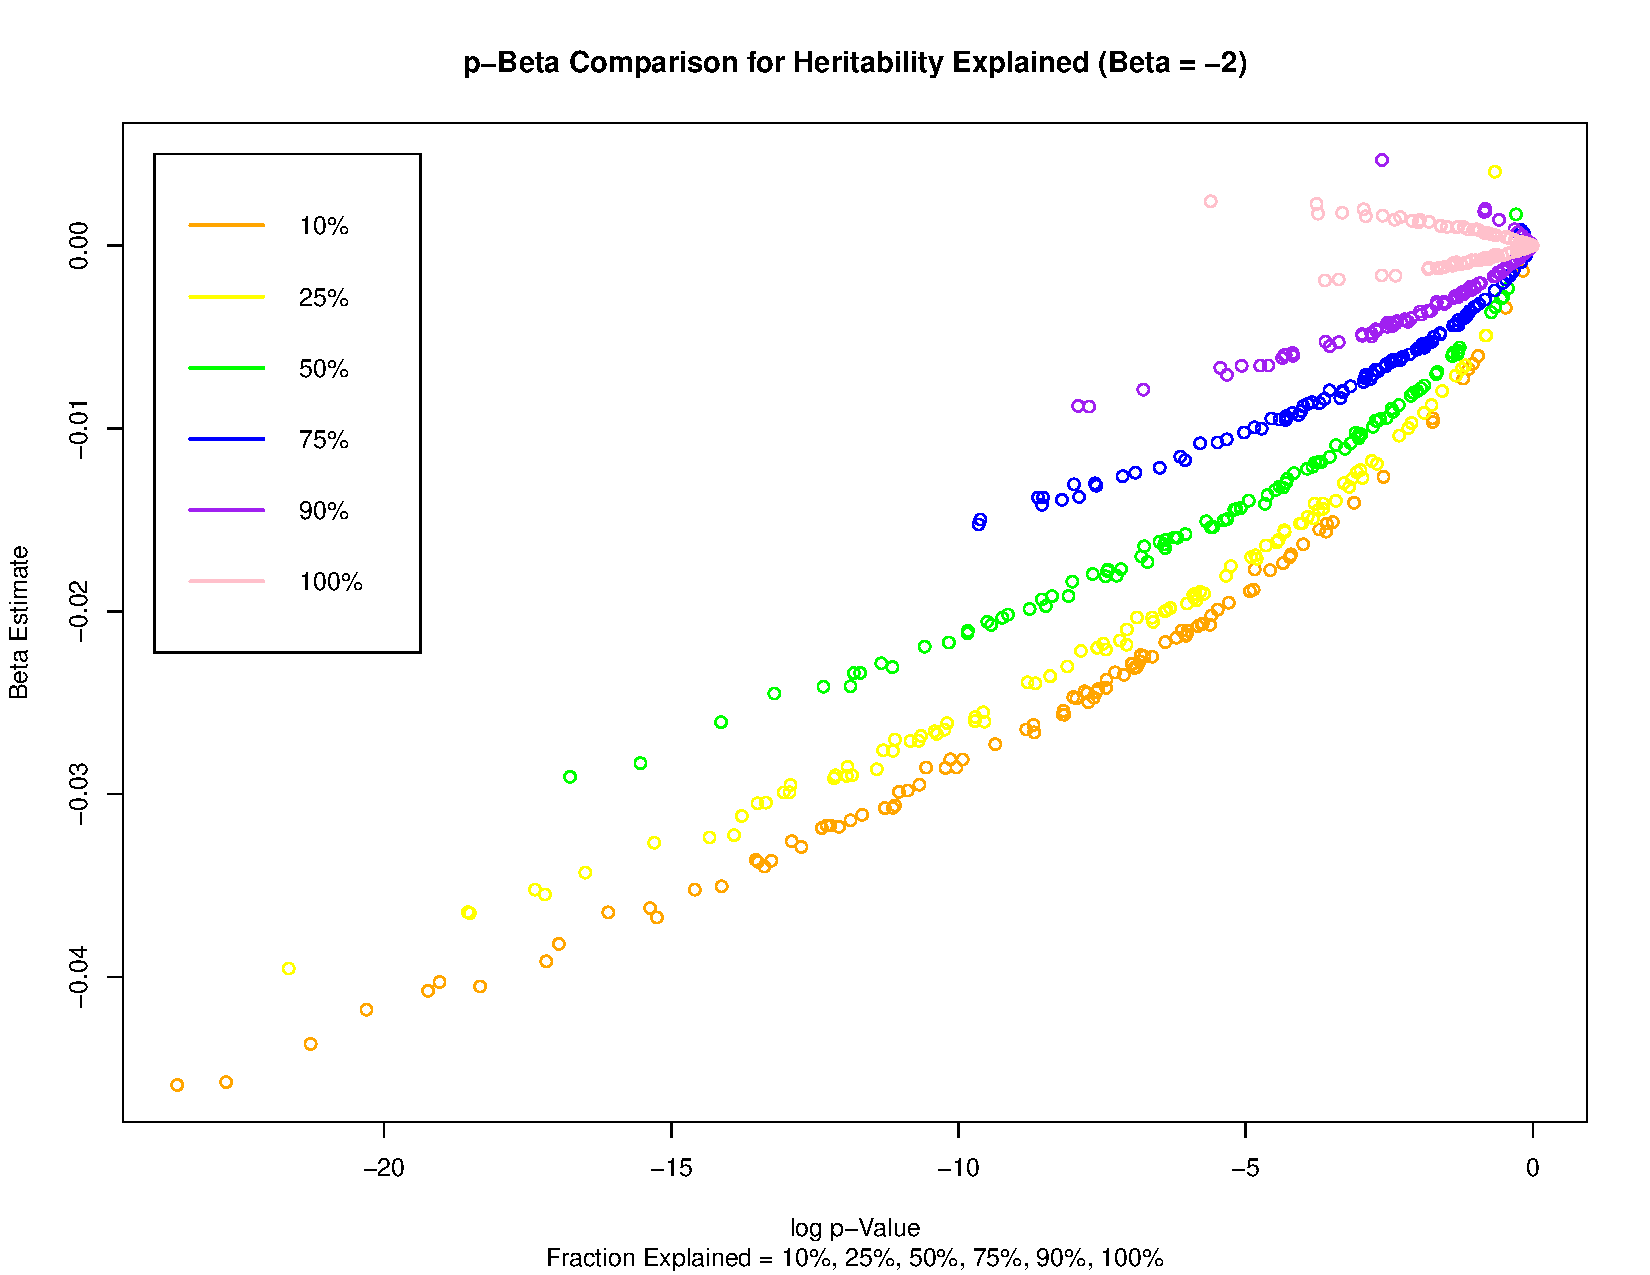
\includegraphics[scale=0.5]{Understanding B/Constant Beta.pdf}

Here, I hold the effect sizes constant, and alter the frequencies.

\end{document}
